\subsection{Example 1}
$C_t=2.2\mathrm{mF}$, $L_t=1.8\mathrm{mH}$, $R_t=0.2\Omega$

\begin{equation}
A=\begin{bmatrix}
    0& \frac{1}{C_t}\\
    -\frac{1}{L_t}& -\frac{-R_t}{L_t}    
\end{bmatrix},\,
B_w=\begin{bmatrix}
    -\frac{1}{C_t}\\
    0    
\end{bmatrix},\,
C=\begin{bmatrix}
    1& 0\\    
    1& 0\\    
    0& 1    
\end{bmatrix}
\end{equation}

\begin{figure}[!htb]
    \centering
    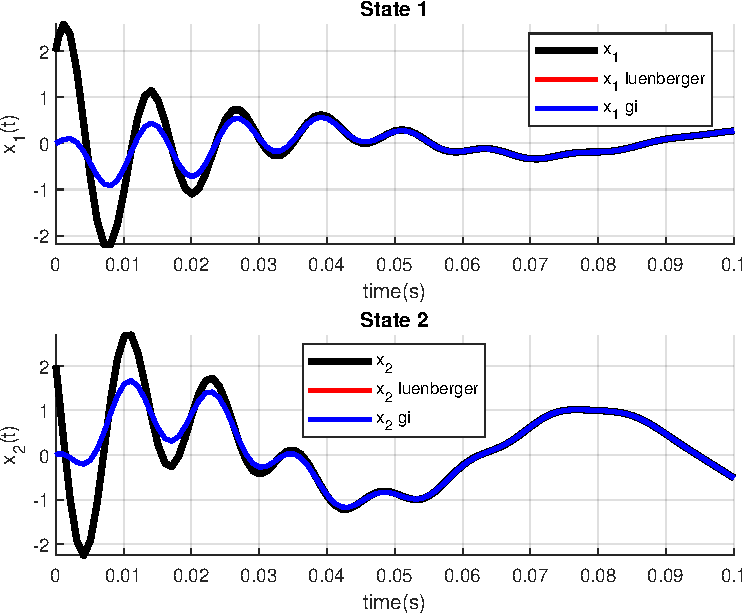
\includegraphics[width=0.85\linewidth]{img/ex1_states1}
    \caption{States}
    \label{fig:ex1_states1}
\end{figure}

\begin{figure}[!htb]
    \centering
    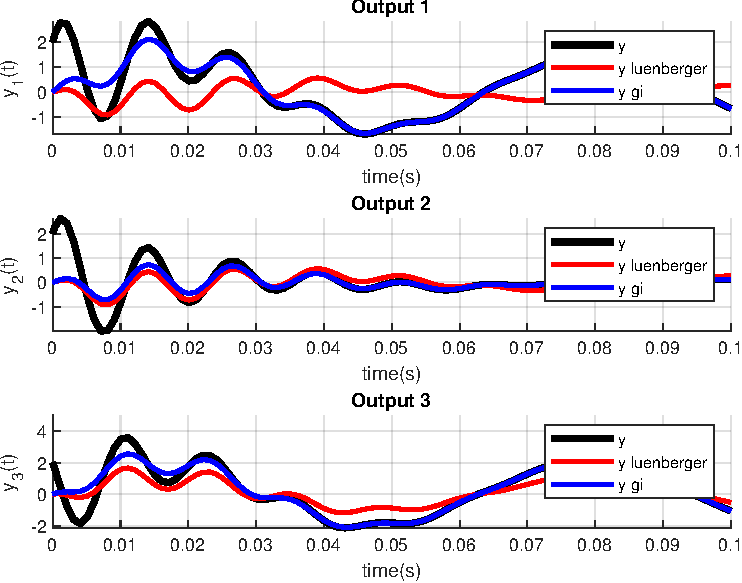
\includegraphics[width=0.85\linewidth]{img/ex1_outputs}
    \caption{Outputs}
    \label{fig:ex1_outputs}
\end{figure}

\begin{figure}[!htb]
    \centering
    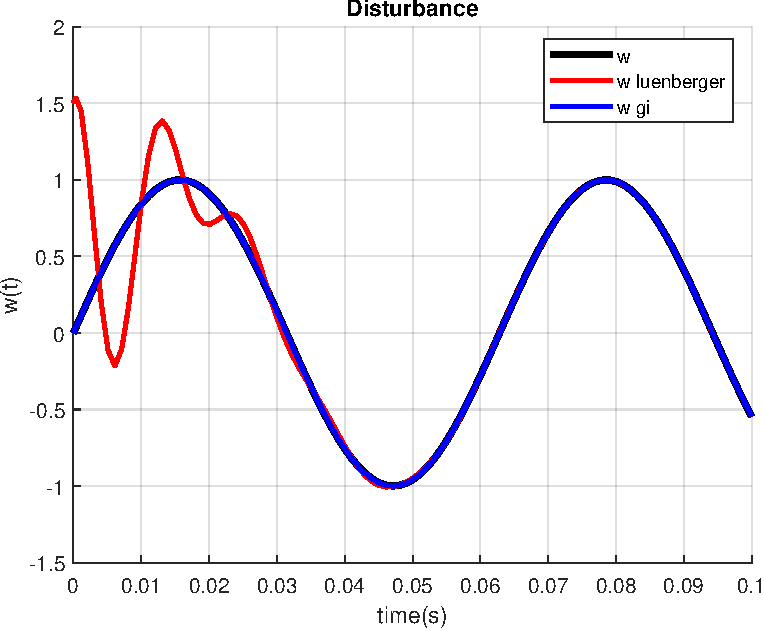
\includegraphics[width=0.85\linewidth]{img/ex1_disturbance}
    \caption{Disturbance}
    \label{fig:ex1_disturbance}
\end{figure}


% %%%%%%%%%%%%%%%%%%%%%%%%%%%%%%%%%%%%%%%%%%%%%%%%%%%%%%%%%%%%%
\subsection{Example 2}

\begin{figure}[!htb]
    \centering
    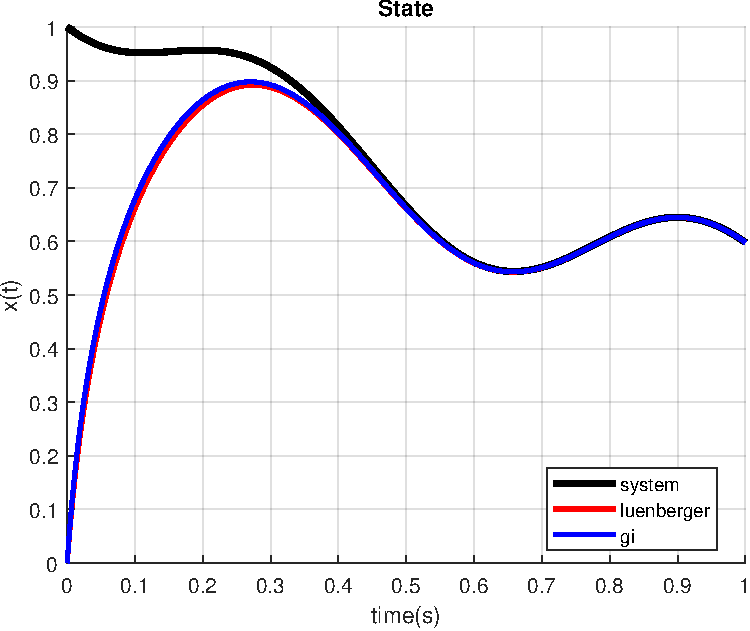
\includegraphics[width=0.85\linewidth]{img/ex2_states1}
    \caption{States}
    \label{fig:ex2_states1}
\end{figure}

\begin{figure}[!htb]
    \centering
    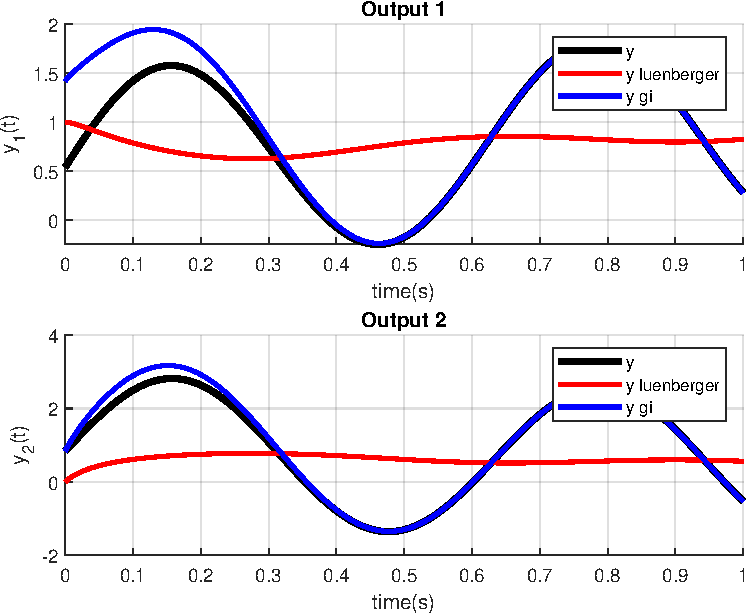
\includegraphics[width=0.85\linewidth]{img/ex2_outputs}
    \caption{Outputs}
    \label{fig:ex2_outputs}
\end{figure}

\begin{figure}[!htb]
    \centering
    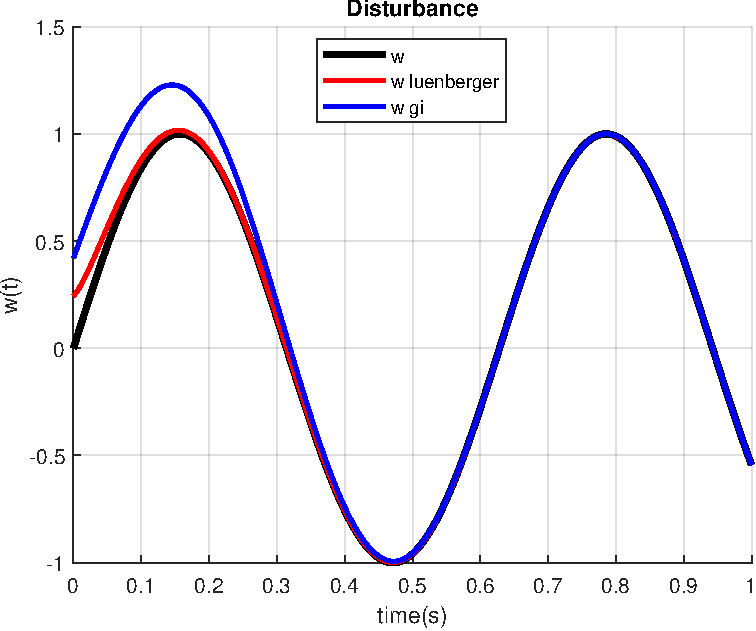
\includegraphics[width=0.85\linewidth]{img/ex2_disturbance}
    \caption{Disturbance}
    \label{fig:ex2_disturbance}
\end{figure}
The following nonlinear system is given,
\begin{equation*}
        \dot{x}=-x^2+w
    \end{equation*}
where outputs are chosen as,
    \begin{equation*}
        \begin{bmatrix}
            y_1\\y_2
        \end{bmatrix}=
        \begin{bmatrix}
            \cos(x)\\\sin(x)
        \end{bmatrix}+\begin{bmatrix}
            1\\2
        \end{bmatrix}w
    \end{equation*}
The matrices after linearization are,
 \begin{equation*}
    \begin{split}
        A(x)&=\frac{d(-x^2)}{dx}\Bigg|_{x=\hat{x}}=-2\hat{x}\\
        B(x)&=1\\
        C(x)&=\begin{bmatrix}
            -\sin(\hat{x})\\\cos(\hat{x})
        \end{bmatrix}
    \end{split}
\end{equation*}
and,
    \begin{equation*}
    \begin{split}
        A(x)-L(x)C(x)&=-2\hat{x}-\begin{bmatrix}l_1& l_2
        \end{bmatrix}\begin{bmatrix}
            -\sin(\hat{x})\\\cos(\hat{x})
        \end{bmatrix}=\lambda\\
        \lambda&=-2\hat{x}+l_1\sin(\hat{x})-l_2\cos(\hat{x})
    \end{split}
    \end{equation*}

The $B-LD_w=0$ condition is satisfied via,
    \begin{equation*}
    \begin{split}
        1-\begin{bmatrix}l_1& l_2
        \end{bmatrix}\begin{bmatrix}1\\2
        \end{bmatrix}&=0\\
        1-l_1-2l_2&=0\\
        l_1&=1-2l_2
    \end{split}
    \end{equation*}
and the projection is calculated as,
    \begin{equation*}
        \Pi=\begin{bmatrix}
            \sin(x)^2& -\sin(x)\cos(x)\\
            -\sin(x)\cos(x)& \cos(x)^2
        \end{bmatrix}
\end{equation*}
Hence,
\begin{equation*}
    \begin{split}
        \lambda&=-2\hat{x}+l_1\sin(\hat{x})-l_2\cos(\hat{x})\\
        \lambda&=-2\hat{x}-2l_2\sin(\hat{x})+\sin(\hat{x})-l_2\cos(\hat{x})\\
        \lambda+2\hat{x}-\sin(\hat{x})&=-2l_2\sin(\hat{x})-l_2\cos(\hat{x})\\
        \lambda+2\hat{x}-\sin(\hat{x})&=l_2(-2\sin(\hat{x})-\cos(\hat{x}))\\
        l_2&=\frac{\lambda+2\hat{x}-\sin(\hat{x})}{-2\sin(\hat{x})-\cos(\hat{x})}
    \end{split}
\end{equation*}
is obtained.